% figures are
%      Overview: brief input (cf 0 is 1. cf 1 is 2. length is 1.) *** DONE *** 
%                brief output (some of the deduced facts containing cp T and cpNote Ts) *** DONE ***
%      Represenation of Music: One interval in sheet music notation to visually explain cf, cp etc. 
%                              Other parts of the definitions if required
%      Enforcement: judgeCP code snippets as needed

% Depending on which note we choose to be the note 0, the note representation part need to be updated (note 0 is C2 etc)

\section{Design and Implementation}
\label{sec:dusa-implementation}

\textcolor{red}{Carlo: I am temporarily holding a lock on this section}

CounterChoice centers around a Dusa logic program that encodes the rules of first-species counterpoint as constraints between a cantus firmus and a counterpoint melody represented as logical predicates (Figure~\ref{fig:dusa-predicates}). For a fixed cantus firmus, solutions of this Dusa program contain valid counterpoint lines for the given melody.


\begin{figure}
\begin{tabular}{l|l}
\textbf{Predicate} & \textbf{Meaning} \\ \hline
\verb|cf T is N| & \verb|T|\textsuperscript{th} note of c.f. has pitch \verb|N| \\
\verb|length T| & c.f. ends on \verb|T|\textsuperscript{th} note \\
\verb|cpNote T is N| & \verb|T|\textsuperscript{th} note of c.p. has pitch \verb|N| \\
\verb|interval I is N| & \verb|I| is a consonant interval of size \verb|N| \\
\verb|cp T is? I| & \verb|T|\textsuperscript{th} note of c.p. is \verb|I| above \verb|cf T| \\
\verb|cpMovement T is N| & \verb|T|\textsuperscript{th},$(\mathtt{T}+1)$\textsuperscript{st} c.p. notes are \verb|N| apart \\
\verb|leap T| & \verb|T|\textsuperscript{th},$(\mathtt{T}+1)$\textsuperscript{st} c.p. notes $>1$ apart
\end{tabular}
\caption{Main Dusa predicates and their meanings.}
\label{fig:dusa-predicates}
\end{figure}


We represent the cantus firmus as a functional predicate \verb|cf T is N| mapping each ``time'' $\mathtt{T}\in\{0,1,\dots\}$ to numbers $\mathtt{N}\in\{0,1,\dots,7\}$ representing one octave of the diatonic scale C4 (when $\mathtt{N}=0$), D4, \dots, B4, C5 (when $\mathtt{N}=7$), along with a predicate \verb|length T| specifying the final time step of the given melody. Note that ``time \verb|T|'' simply refers to the \verb|T|\textsuperscript{th} note of the melody, as the two melodies move in lock-step and we do not encode any information about duration.

\begin{verbatim}
  cf 0 is 1.
  cf 1 is 4.
  cf 2 is 3.
  ...
  cf 8 is 4.
  length is 8.
\end{verbatim}

We likewise represent the counterpoint melody as a functional predicate \verb|cpNote T is N| with $\mathtt{N}\in\{0,1,\dots,13\}$.

The remainder of the Dusa predicates and rules, listed in Figures~\ref{fig:dusa-predicates} and \ref{fig:dusa-forbidden}, enforce various properties of \verb|cpNote| drawn from a mixture of Fux's rules of first species counterpoint~\cite{fux-cp} and ToneSavvy's interactive counterpoint exercises~\cite{tonesavvy}. Some of these properties are \emph{vertical} in that they relate the values of \verb|cf T| and \verb|cpNote T| at a single \verb|T|, whereas others are \emph{horizontal} in that they relate to the motion of one or both melodies across multiple consecutive time steps.



\paragraph{Intervals and consonance}

A key rule of counterpoint is that \emph{the interval between the cantus firmus and counterpoint must be consonant}, namely a unison, third, fifth, sixth, or octave. For simplicity we assume that the counterpoint melody is always \emph{above} the cantus firmus by one of these intervals, and we do not distinguish between major/minor or perfect/augmented/diminished intervals.

We use the functional predicate \verb|interval I is N| as a ``lookup table'' mapping the names of consonant intervals to pitch differences (e.g., the pitch a \verb|third| above \verb|N| is $\texttt{N}+2$).

\begin{verbatim}
  interval unison is 0.
  interval third is 2.
  interval fifth is 4.
  interval sixth is 5.
  interval octave is 7.
\end{verbatim}

Because the consonance requirement dramatically reduces the state space---it restricts the counterpoint melody to one of five possible values per time step---we found it useful to center our Dusa implementation around this restriction. We specify the predicate \verb|cp T is? I| as an open choice requiring each time step to map to one of the five consonant intervals.
%
\begin{verbatim}
  cp T is? I :-
    cf T is _,
    interval I is _.
\end{verbatim}
%
The wildcard premise \verb|cf T is _| ensures that \verb|cp T| is only required to be defined for the same \verb|T| as the predicate \verb|cf|.

For each generated fact \verb|cp T is I| we then define the counterpoint note \verb|cpNote T| to be the correct interval above \verb|cf T|, using the \verb|interval| predicate defined above.

\begin{verbatim}
  cpNote T is (plus N (interval I)) :-
    cp T is I,
    cf T is N.
\end{verbatim}



\paragraph{Other vertical constraints}

In addition to the consonance requirement at every time step, there are several other vertical constraints governing harmony at certain times. For instance, \emph{the starting and ending intervals must each be a unison or an octave}. We represent these constraints as closed choices that refine the general open choice \verb|cp T is? I|.

\begin{verbatim}
  cp 0 is {unison, octave}.
  cp length is {unison, octave}.
\end{verbatim}

The final vertical constraint is that \emph{the unison is not allowed anywhere else}. We specify this as a \verb|#forbid| declaration ruling out any solutions in which the fact \verb|unisoninMiddle T| is derivable for any \verb|T|. This fact is in turn derivable whenever there is a time step $0<\mathtt{T}<\mathtt{length}$ with \verb|cp T is unison|.

\begin{verbatim}
  #forbid unisoninMiddle _.
  unisoninMiddle T :-
    cf T is _,
    T > 0,
    T < length,
    cp T is unison.
\end{verbatim}



\paragraph{Parallel fifths and octaves}

The remaining constraints are horizontal, in the sense that they govern multiple consecutive time steps. Most of these constraints are negative and thus easily specified as \verb|#forbid| declarations (see Figure~\ref{fig:dusa-forbidden}).

The simplest of these is the restriction on parallel fifths: \emph{if the previous interval is a fifth, the next interval should not also be a fifth}. As with \verb|unisoninMiddle|, it is easy to define a predicate \verb|parallelFifth T| which holds exactly when this restriction is violated, and \verb|#forbid| it from ever holding.

\begin{verbatim}
  #forbid parallelFifth _.
  parallelFifth T :-
    cp T is fifth,
    cp (suc T) is fifth.
\end{verbatim}

A similar restriction applies to parallel octaves.

\begin{verbatim}
  #forbid parallelOctave _.
  parallelOctave T :-
    cp T is octave,
    cp (suc T) is octave.
\end{verbatim}



\paragraph{Counterpoint movement}

The next constraint is a positive one: \emph{the counterpoint melody should move in steps, or in leaps of a third, fourth, fifth, or sixth}. It is possible to encode such a condition directly in Dusa, e.g.\ by \verb|#demand|ing a predicate that holds only when the entire melody satisfies this condition. However, such an encoding requires Dusa to generate an entire candidate melody before checking for validity, whereas negative \verb|#forbid| constraints allow Dusa to quickly prune invalid regions of the search space.

For this reason, we rephrase the constraint as: \emph{the counterpoint melody must not stay stationary, nor move by more than a sixth}. We define a predicate \verb|invalidCPMovement T| which holds when one of these forbidden movements occurs between times \verb|T| and $\mathtt{T}+1$, and \verb|#forbid| it.

\begin{verbatim}
  #forbid invalidCPMovement _.
  invalidCPMovement T :-
    cf T is _,
    cpMovement T > 5.
  invalidCPMovement T :-
    cf T is _,
    cpMovement T is 0.
\end{verbatim}

The above rules are stated in terms of the auxiliary functional predicate \verb|cpMovement T is N| which holds when the distance (in absolute value) between \verb|cpNote T| and \verb|cpNote (suc T)| is \verb|N|. This predicate is marked as \verb|#lazy| so that it is only computed when required as a premise.

\begin{verbatim}
  #lazy cpMovement
  cpMovement T is (minus N2 N1) :-
    cpNote T is N1,
    cpNote (suc T) is N2,
    N2 >= N1.
  cpMovement T is (minus N1 N2) :-
    cpNote T is N1,
    cpNote (suc T) is N2,
    N1 > N2.
\end{verbatim}



\paragraph{Consecutive leaps}

The next several constraints further limit when the counterpoint melody can move in leaps. First, \emph{the counterpoint melody must not contain multiple successive large leaps (fifths or sixths) in the same direction}. Given that we have already ruled out leaps greater than a sixth, this condition is equivalent to checking for leaps greater than a fourth (i.e., greater than distance $3$).

We \verb|#forbid| two separate predicates \verb|twoLargeLeapsUp T| and \verb|twoLargeLeapsDown T| which hold when the counterpoint melody moves by large leaps in the same direction between times $\mathtt{T}\to(\mathtt{T}+1)$ and $(\mathtt{T}+1)\to(\mathtt{T}+2)$.

\begin{verbatim}
  #forbid twoLargeLeapsUp _.
  twoLargeLeapsUp T :-
    cf T is _,
    cpNote (suc T) > plus 3 (cpNote T),
    cpNote (plus T 2) > plus 3 (cpNote (suc T)).

  #forbid twoLargeLeapsDown _.
  twoLargeLeapsDown T :-
    cf T is _,
    plus 3 (cpNote (suc T)) < cpNote T,
    plus 3 (cpNote (plus T 2)) < cpNote (suc T).
\end{verbatim}

Another constraint is that \emph{the counterpoint melody cannot have more than three leaps (movements greater than a step) in a row}. We define a \verb|#lazy| auxiliary predicate \verb|leap T| to hold when \verb|cpNote T| and \verb|cpNote (suc T)| differ by more than $1$.

\begin{verbatim}
  #lazy leap
  leap T :-
    cpMovement T > 1.
\end{verbatim}

We then \verb|#forbid fourLeaps T|, or four consecutive leaps between times \verb|T| and $\mathtt{T}+4$.

\begin{verbatim}
  #forbid fourLeaps _.
  fourLeaps T :-
    cf T is _,
    leap T,
    leap (plus T 1),
    leap (plus T 2),
    leap (plus T 3).
\end{verbatim}



\textcolor{red}{Carlo: I am here}

\paragraph{Direct fifths and octaves}

\begin{verbatim}
  #forbid directFifth _.
  directFifth T :-
    cf T is _,
    cp (suc T) is fifth,
    directMotion T,
    leap T.
\end{verbatim}

\begin{verbatim}
  #forbid directOctave _.
  directOctave T :-
    cf T is _,
    cp (suc T) is octave,
    directMotion T,
    leap T.
\end{verbatim}

\begin{verbatim}
#lazy directMotion
directMotion T :-
  cf T is _,
  cf (suc T) > cf T,
  cpNote (suc T) > cpNote T.

directMotion T :-
  cf T is _,
  cf (suc T) < cf T,
  cpNote (suc T) < cpNote T.
\end{verbatim}

TODO add directMotion, directFifth, directOctave to figures

\begin{figure}
\begin{tabular}{l|l}
\textbf{Predicate} & \textbf{Meaning} \\ \hline
\verb|unisonInMiddle T| & interval $\mathtt{T}\not\in\{0,\texttt{length}\}$ is unison \\
\verb|parallelFifth T| & intervals $\mathtt{T},(\mathtt{T}+1)$ both fifths \\
\verb|parallelOctave T| & intervals $\mathtt{T},(\mathtt{T}+1)$ both octaves \\
\verb|invalidCPMovement T| & invalid c.p. movement $\mathtt{T}\to(\mathtt{T}+1)$ \\
\verb|twoLargeLeapsUp T| & c.p. leaps up 5\textsuperscript{th}/6\textsuperscript{th} $\mathtt{T}\to(\mathtt{T}+2)$ \\
\verb|twoLargeLeapsDown T| & c.p. leaps down 5\textsuperscript{th}/6\textsuperscript{th}\dots \\
\verb|fourLeaps T| & c.p. $4\times$ leaps $\mathtt{T}\to(\mathtt{T}+4)$
\end{tabular}
\caption{\texttt{\#forbid}den Dusa predicates.}
\label{fig:dusa-forbidden}
\end{figure}

\paragraph{Cadence}

\begin{verbatim}
  #demand cadenceStepwiseContrary.

  cadenceStepwiseContrary :-
    suc T is length,
    suc (cf T) == cf length,
    cpNote T == suc (cpNote length).

  cadenceStepwiseContrary :-
    suc T is length,
    cf T == suc (cf length),
    suc (cpNote T) == cpNote length.
\end{verbatim}

TODO add cadenceStepwiseContrary to first figure?

TODO not yet mentioning 'at'

TODO subsection structure TBD

\subsection{Old Text}

\subsubsection{Horizontal Constraints}
Rules grouped together in this category concern the movement of counterpoint notes, or the movement of intervals in consequent bars. This means that they can be thought of as governing the melody and the harmony together.

The rules are as follows:
\begin{itemize}
  \item Ends with a cadence: TODO
  \item If the notes in cantus firmus and counterpoint melodies move in the same direction, and there is a \texttt{leap} in the counter-melody going from time step \texttt{T} to \texttt{T+1}, the resulting interval should not be a \texttt{fifth} or an \texttt{octave} (Direct fifths or octaves).
\end{itemize}


\subsubsection{Enforcing the Rules}

The task is to find valid \texttt{cp} values for all time steps \texttt{T} for the given \texttt{cf} values. Therefore, we introduced Dusa rules to generate \texttt{cp}s and ensure that only valid ones are accepted:

Also, facts and rules used only as intermediate steps such as \texttt{movement} are all made to be lazy predicates. This is to prevent redundant deductions in the output.

\paragraph{Cadence - Unison}

The rule states that if the cantus firmus melody ends with an upwards motion, the counterpoint melody should fall in contrary motion from a \texttt{third} to a \texttt{unison}.

The check for upward motion in the last two notes of cantus firmus is done by \texttt{(cf (suc T)) > (cf T)}, and if \texttt{cp T} is not \texttt{third} when there is upward movement, \texttt{judgeCP} evaluates to \texttt{bad}. The Dusa rule below sets the \texttt{cp length} to \texttt{unison} for the last note. Note that we assumed that the user will enter a valid ending for the cantus firmus, eg. not oblique motion.



\subsection{Optimization}
The above approach using \texttt{judgeCP} worked well with small cantus firmi, but solution generation hit a bottleneck around 12 note pieces and failed to produce a solution reliably for anything longer.\par Therefore, we reexamined the Dusa code and optimized it in the following ways.

\subsubsection{Refactoring}

We tried to see how the implementation can be made more efficient while preserving the original functionality. For this purpose, we made some changes to reduce the number of choices and deductions by Dusa, and rearranged the rule-checking without using \texttt{judgeCP}.

\paragraph{Mentioning Variables}
One feature of Dusa is that the variables used on the conclusion of a rule need to be mentioned by one of the premises on the right hand side. If the value of the variable is not important, it is possible to use a wildcard, \texttt{\_}, in the premise for mentioning. Wildcards work by matching all possible values for that variable.

In \texttt{judgeCP T I} rules, we check whether \texttt{T} is a valid time step with the premise \texttt{cp T is \_}. Although the wildcard discards the matched value, the system must still derive all matching \texttt{cp T} facts, increasing the deduction space. Since \texttt{cp} and \texttt{cf} exist for the same time steps, changing every instance of \texttt{cp T is \_} that is used only to mention \texttt{T} with the premise \texttt{cf T is \_} preserves the same functionality and is much lighter than \texttt{cp} to create each time.

\paragraph{Forbid Declarations}
Although using a closed rule for \texttt{judgeCP} was more efficient than the initial version, two issues remained. First, all rules are enforced by a single rule named \texttt{judgeCP}. And second, essentially, the only choice needed is \texttt{cp T is? I}; that is, even if we reduced the number of choices with the introduction of the closed rule, we should be able to eliminate choices for anything besides \texttt{cp} entirely. And our solution was to transform \texttt{judgeCP} from a rule into separate  facts as follows:
\begin{verbatim}
  cadenceNotThirdUnison (minus length 1) I :-
  (minus length 1) is T,
  cp T is I,
  (cf (suc T)) > (cf T),
  I != third.
  ...
  #forbid cadenceNotThirdUnison _ _.
\end{verbatim}
At the end of the code, we include all violating facts as "forbid declarations" with their unique names. This approach has three benefits:
\begin{itemize}
  \item Having rules separately makes it easy to understand/debug since rule names are visible.
  \item It makes it easy for anyone who wants to adjust the ruleset to easily select which rules they want to apply.
  \item Since \texttt{judgeCP} is eliminated, dependencies of some of the facts are reduced. In the previous version, all rules needed to have an \texttt{N} and \texttt{I} component but not anymore.
\end{itemize}

With these final changes, we reduced the system with multiple choices into a modular one-open-choice model while keeping the solution set intact. The initial bottleneck of 12 notes also increased to more than 30. However, for very long pieces, the code still takes up a lot of time due to search space getting exponentially? larger as T increases. For that reason, we tried another approach to tackle longer pieces as the next step.





\subsection{External support}

\subsubsection{Alternative Approach: Divide-and-Conquer}
To circumvent/work around the bottleneck of 12 notes, the idea we came up with is to divide the cantus firmus into smaller chunks, solve them, and then assemble those solutions together to get the final solution. This divide and conquer approach has the advantage of resembling how humans compose counterpoint for specific melody parts and put them together, instead of treating each note and phrase with the same importance, as well as the advantage of bypassing the large search space.


\paragraph{Overlapping Segments}
Checks for the consecutive notes need a special treatment in this method to see that the end and starting \texttt{cp}s are compatible in the chunks. To tackle this, after creating the solution for the first chunk, we selected the consecutive chunks to have an overlap of 3 notes (first solving for \texttt{cf 0} to \texttt{cf 7}, then \texttt{cf 5} to \texttt{cf 12} and so on). At the same time, the intervals found for the last 3 steps were written as facts to the Dusa code of the next chunk's solver such as \begin{verbatim}
  cp 5 is fifth.
  cp 6 is third.
  cp 7 is third.
\end{verbatim} to prevent duplicate solutions for overlapping steps.

\paragraph{Specialized Solvers}
We used three different Dusa codes to generate solutions to the beginning, middle, and end chunks to account for the ending cadence rule, the starting interval rule, and the "No Unison in Middle" rules.

%\paragraph{}
%We also called Dusa asynchronously in JavaScript to enable interruptions to calls of \texttt{dusa.solve()}. When Dusa generates a solution, a common problem was when it entered a sub-optimal branch during its deductions, it got stuck there. We worked around this by interrupting the generation after a set time (2s) and rerunning it for the set number of attempts (10). 2s were chosen since the typical time Dusa takes to find a solution for an 8 note piece is under 0.5ms. Also, normally for another language, rerunning the exact solver with the exact input would yield the same results, but this is where Dusa's undeterministic nature comes in handy.

The results of this implementation were generally good. While it sometimes got stuck on a random chunk before creating a full solution, it was quite fast when it did find a solution. Further improvements can be made to this approach, but since the normal optimizations made the code handle more than 20 notes comfortably, and taking care of the longer pieces is going a little out of scope for this project, we decided to move on to the validation of generated solutions.

\subsubsection{Validating the Solution}
To test the solutions, we wrote a validation code in JavaScript that checks the solutions obtained from Dusa. The rules of counterpoint were rewritten in JavaScript for testing. Then, solutions are iterated using
\begin{verbatim}
  const iterator = dusa.solve();
  const result = iterator.next();
\end{verbatim}, and various values from the solution are fetched using \texttt{solution.lookup()} and compared with their expected values. The solutions have passed the tests we conducted.

% I don't know if we will use the web version or JavaScript API in the final version so I am leaving this commented out for now. Below is how the original version handled it..
% We call dusa.solution() inside Java Script to get one solution Dusa generates, and then convert that solution into MIDI format for being able to listen to it.

\subsubsection{Other tools}

% removed this figure for now

%\begin{figure}[H]
%    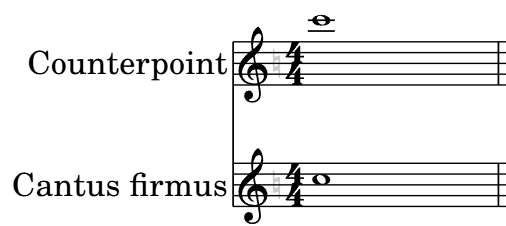
\includegraphics[width=0.5\linewidth]{interval-octave.png}
%\end{figure}
% In this figure, cantus firmus has a C5, counterpoint has a C6, and they create an \texttt{octave} together. In our representation, this is expressed as: 
%\begin{verbatim}
%    cf 0 is 0.
%    cp 0 is octave.
%    cpNote 0 is 7.
%\end{verbatim}

